\begin{figure*}[t]
\centering
\resizebox{\textwidth}{!}{%
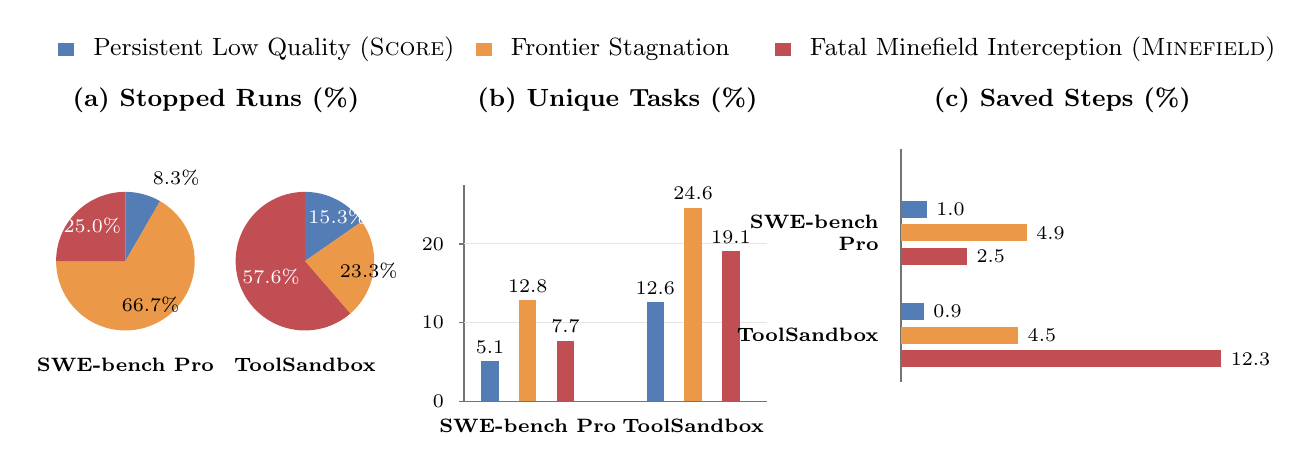
\begin{tikzpicture}[
    font=\small,
    value/.style={font=\scriptsize, inner sep=1.5pt},
    benchmark/.style={font=\scriptsize\bfseries},
    panel/.style={font=\small\bfseries},
    tick/.style={font=\scriptsize, black},
    axis/.style={draw=black!55, line width=0.5pt},
    gridline/.style={draw=black!10, line width=0.4pt},
]
    \definecolor{ScoreBlue}{RGB}{84,124,181}
    \definecolor{StagnationOrange}{RGB}{235,153,73}
    \definecolor{MinefieldRed}{RGB}{193,78,82}

    % Shared legend
    \fill[ScoreBlue] (0.05,4.55) rectangle ++(0.20,-0.16);
    \node[anchor=west] at (0.37,4.47) {Persistent Low Quality (\textsc{Score})};
    \fill[StagnationOrange] (5.35,4.55) rectangle ++(0.20,-0.16);
    \node[anchor=west] at (5.67,4.47) {Frontier Stagnation};
    \fill[MinefieldRed] (9.15,4.55) rectangle ++(0.20,-0.16);
    \node[anchor=west] at (9.47,4.47) {Fatal Minefield Interception (\textsc{Minefield})};

    % (a) Composition of stopped runs
    \node[panel] at (2.05,3.82) {(a) Stopped Runs (\%)};

    % SWE-bench Pro pie
    \fill[ScoreBlue] (0.90,1.78) -- ++(90:0.88)
        arc[start angle=90, end angle=60, radius=0.88] -- cycle;
    \fill[StagnationOrange] (0.90,1.78) -- ++(60:0.88)
        arc[start angle=60, end angle=-180, radius=0.88] -- cycle;
    \fill[MinefieldRed] (0.90,1.78) -- ++(-180:0.88)
        arc[start angle=-180, end angle=-270, radius=0.88] -- cycle;
    \node[value, anchor=west] at (1.19,2.84) {8.3\%};
    \node[value] at (1.22,1.23) {66.7\%};
    \node[value, text=white] at (0.48,2.23) {25.0\%};
    \node[benchmark] at (0.90,0.46) {SWE-bench Pro};

    % ToolSandbox pie
    \fill[ScoreBlue] (3.18,1.78) -- ++(90:0.88)
        arc[start angle=90, end angle=34.835, radius=0.88] -- cycle;
    \fill[StagnationOrange] (3.18,1.78) -- ++(34.835:0.88)
        arc[start angle=34.835, end angle=-49.127, radius=0.88] -- cycle;
    \fill[MinefieldRed] (3.18,1.78) -- ++(-49.127:0.88)
        arc[start angle=-49.127, end angle=-270, radius=0.88] -- cycle;
    \node[value, text=white] at (3.59,2.35) {15.3\%};
    \node[value] at (3.99,1.66) {23.3\%};
    \node[value, text=white] at (2.75,1.58) {57.6\%};
    \node[benchmark] at (3.18,0.46) {ToolSandbox};

    % (b) Unique-task coverage
    \node[panel] at (7.15,3.82) {(b) Unique Tasks (\%)};
    \draw[axis] (5.20,0) -- (9.05,0);
    \draw[axis] (5.20,0) -- (5.20,2.75);
    \foreach \y/\label in {0/0, 1.0/10, 2.0/20} {
        \draw[axis] (5.14,\y) -- (5.20,\y);
        \node[tick, anchor=east] at (5.07,\y) {\label};
    }
    \draw[gridline] (5.20,1.0) -- (9.05,1.0);
    \draw[gridline] (5.20,2.0) -- (9.05,2.0);

    % SWE-bench Pro bars
    \fill[ScoreBlue] (5.42,0) rectangle (5.64,0.513);
    \fill[StagnationOrange] (5.90,0) rectangle (6.12,1.282);
    \fill[MinefieldRed] (6.38,0) rectangle (6.60,0.769);
    \node[value, anchor=south] at (5.53,0.55) {5.1};
    \node[value, anchor=south] at (6.01,1.32) {12.8};
    \node[value, anchor=south] at (6.49,0.81) {7.7};
    \node[benchmark] at (6.01,-0.31) {SWE-bench Pro};

    % ToolSandbox bars
    \fill[ScoreBlue] (7.52,0) rectangle (7.74,1.257);
    \fill[StagnationOrange] (8.00,0) rectangle (8.22,2.456);
    \fill[MinefieldRed] (8.48,0) rectangle (8.70,1.906);
    \node[value, anchor=south] at (7.63,1.30) {12.6};
    \node[value, anchor=south] at (8.11,2.50) {24.6};
    \node[value, anchor=south] at (8.59,1.95) {19.1};
    \node[benchmark] at (8.11,-0.31) {ToolSandbox};

    % (c) Saved steps
    \node[panel] at (12.80,3.82) {(c) Saved Steps (\%)};
    \draw[axis] (10.75,0.25) -- (10.75,3.20);

    % SWE-bench Pro bars
    \fill[ScoreBlue] (10.75,2.33) rectangle (11.08,2.55);
    \fill[StagnationOrange] (10.75,2.03) rectangle (12.35,2.25);
    \fill[MinefieldRed] (10.75,1.73) rectangle (11.59,1.95);
    \node[value, anchor=west] at (11.14,2.44) {1.0};
    \node[value, anchor=west] at (12.41,2.14) {4.9};
    \node[value, anchor=west] at (11.65,1.84) {2.5};
    \node[benchmark, anchor=east, align=right] at (10.59,2.14) {SWE-bench\\ Pro};

    % ToolSandbox bars
    \fill[ScoreBlue] (10.75,1.03) rectangle (11.04,1.25);
    \fill[StagnationOrange] (10.75,0.73) rectangle (12.24,0.95);
    \fill[MinefieldRed] (10.75,0.43) rectangle (14.82,0.65);
    \node[value, anchor=west] at (11.10,1.14) {0.9};
    \node[value, anchor=west] at (12.30,0.84) {4.5};
    \node[value, anchor=west] at (14.88,0.54) {12.3};
    \node[benchmark, anchor=east] at (10.59,0.84) {ToolSandbox};
\end{tikzpicture}%
}
\caption{\textbf{Early-stop behavior and savings by termination criterion.} (a) Stopped-run shares, (b) unique-task coverage, and (c) Saved Steps contributions on ToolSandbox and SWE-bench Pro. Unique-task shares are not additive.}
\label{fig:early_stop}
\end{figure*}
